\documentclass[aspectratio=169]{../latex_main/tntbeamer}  % you can pass all options of the beamer class, e.g., 'handout' or 'aspectratio=43'
\usepackage{dsfont}
\usepackage{bm}
\usepackage[english]{babel}
\usepackage[T1]{fontenc}
%\usepackage[utf8]{inputenc}
\usepackage{graphicx}
\graphicspath{ {./figures/} }
\usepackage{algorithm}
\usepackage[ruled,vlined,algo2e,linesnumbered]{algorithm2e}
\usepackage{hyperref}
\usepackage{booktabs}
\usepackage{mathtools}

\usepackage{amsmath,amssymb}

\DeclareMathOperator*{\argmax}{arg\,max}
\DeclareMathOperator*{\argmin}{arg\,min}

\usepackage{amsbsy}
\newcommand{\vect}[1]{\bm{#1}}
%\newcommand{\vect}[1]{\boldsymbol{#1}}

\usepackage{pgfplots}
\pgfplotsset{compat=1.16}
\usepackage{tikz}
\usetikzlibrary{trees} 
\usetikzlibrary{shapes.geometric}
\usetikzlibrary{positioning,shapes,shadows,arrows,calc,mindmap}
\usetikzlibrary{positioning,fadings,through}
\usetikzlibrary{decorations.pathreplacing}
\usetikzlibrary{intersections}
\pgfdeclarelayer{background}
\pgfdeclarelayer{foreground}
\pgfsetlayers{background,main,foreground}
\tikzstyle{activity}=[rectangle, draw=black, rounded corners, text centered, text width=8em]
\tikzstyle{data}=[rectangle, draw=black, text centered, text width=8em]
\tikzstyle{myarrow}=[->, thick, draw=black]

% Define the layers to draw the diagram
\pgfdeclarelayer{background}
\pgfdeclarelayer{foreground}
\pgfsetlayers{background,main,foreground}

% Requires XeLaTeX or LuaLaTeX
%\usepackage{unicode-math}

\usepackage{fontspec}
%\setsansfont{Arial}
\setsansfont{RotisSansSerifStd}[ 
Path=../latex_main/fonts/,
Extension = .otf,
UprightFont = *-Regular,  % or *-Light
BoldFont = *-ExtraBold,  % or *-Bold
ItalicFont = *-Italic
]
\setmonofont{Cascadia Mono}[
Scale=0.8
]

% scale factor adapted; mathrm font added (Benjamin Spitschan @TNT, 2021-06-01)
%\setmathfont[Scale=1.05]{Libertinus Math}
%\setmathrm[Scale=1.05]{Libertinus Math}

% other available math fonts are (not exhaustive)
% Latin Modern Math
% XITS Math
% Libertinus Math
% Asana Math
% Fira Math
% TeX Gyre Pagella Math
% TeX Gyre Bonum Math
% TeX Gyre Schola Math
% TeX Gyre Termes Math

% Literature References
\newcommand{\lit}[2]{\href{#2}{\footnotesize\color{black!60}[#1]}}

%%% Beamer Customization
%----------------------------------------------------------------------
% (Don't) Show sections in frame header. Options: 'sections', 'sections light', empty
\setbeamertemplate{headline}{empty}

% Add header logo for normal frames
\setheaderimage{
	% 
\includegraphics[height=\logoheight]{figures/TNT_darkv4.pdf}
	
\includegraphics[height=\logoheight]{../latex_main/figures/luh_logo_rgb_0_80_155.pdf}
	% 
\includegraphics[height=\logoheight]{figures/logo_tntluh.pdf}
}

% Header logo for title page
\settitleheaderimage{
	% 
\includegraphics[height=\logoheight]{figures/TNT_darkv4.pdf}
	
\includegraphics[height=\logoheight]{../latex_main/figures/luh_logo_rgb_0_80_155.pdf}
	% 
\includegraphics[height=\logoheight]{figures/logo_tntluh.pdf}
}

% Title page: tntdefault 
\setbeamertemplate{title page}[tntdefault]  % or luhstyle
% Add optional title image here
%\addtitlepageimagedefault{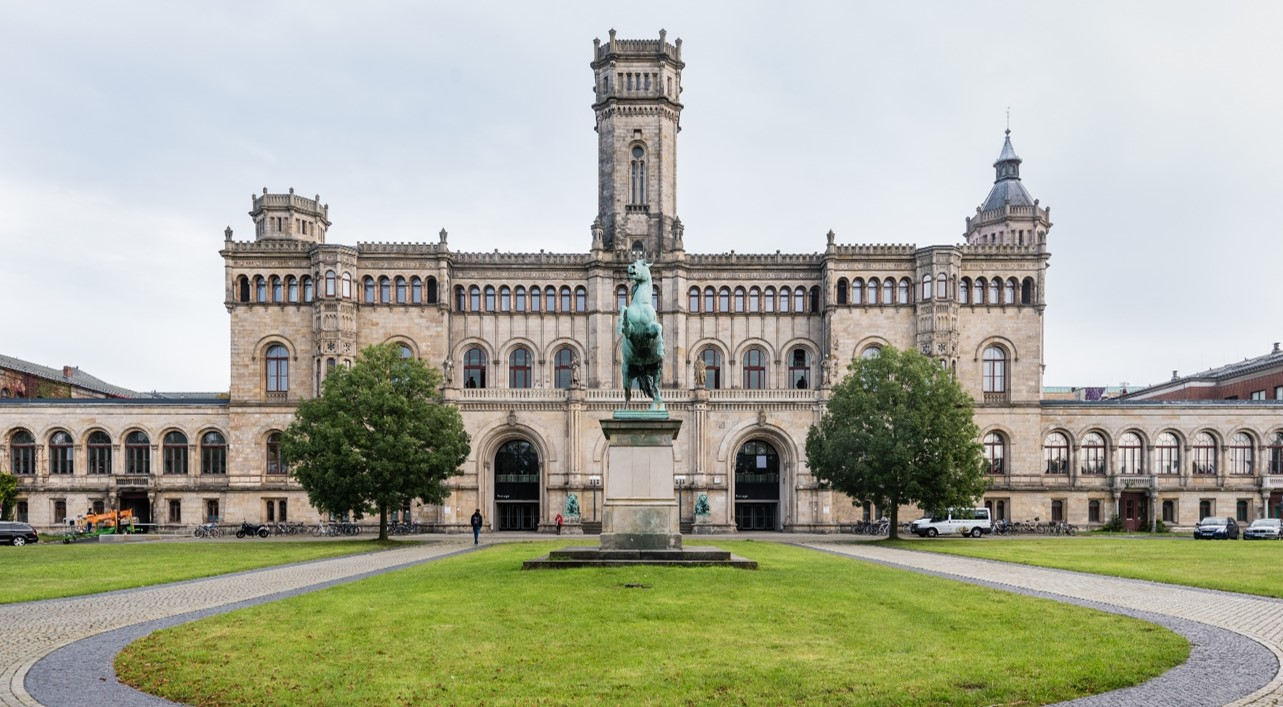
\includegraphics[width=0.65\textwidth]{figures/luh_default_presentation_title_image.jpg}}

% Title page: luhstyle
% \setbeamertemplate{title page}[luhstyle]
% % Add optional title image here
% \addtitlepageimage{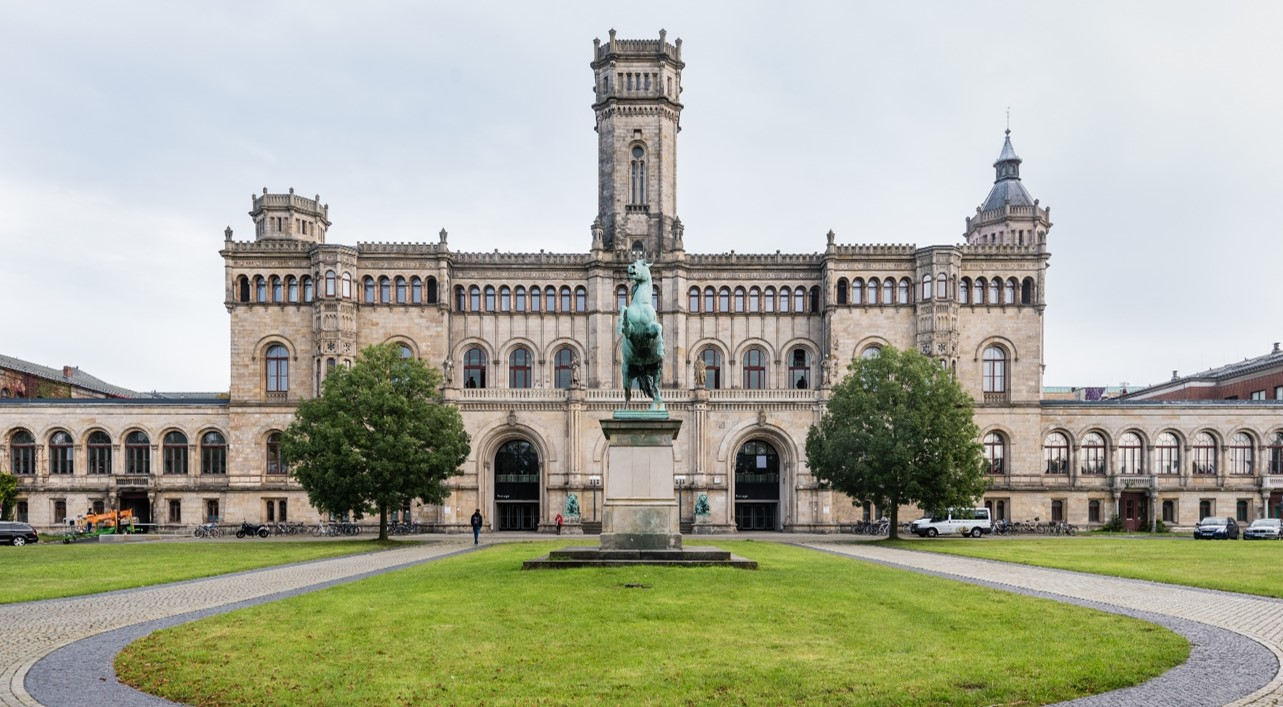
\includegraphics[width=0.75\textwidth]{figures/luh_default_presentation_title_image.jpg}}

\author[Abedjan \& Lindauer]{Ziawasch Abedjan \& Marius Lindauer\\[1em]
	
\includegraphics[height=\logoheight]{../latex_main/figures/luh_logo_rgb_0_80_155.pdf}\qquad
	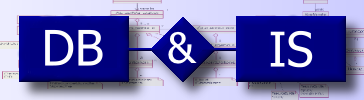
\includegraphics[height=\logoheight]{../latex_main/figures/DBIS_Kurzlogo.png}\qquad

\includegraphics[height=\logoheight]{../latex_main/figures/TNT_darkv4}\qquad

\includegraphics[height=\logoheight]{../latex_main/figures/L3S.jpg}	}
\date{Summer Term 2022; \hspace{0.5em} {
\includegraphics[height=1.5em]{../latex_main/figures/Cc-by-nc-sa_icon.svg.png}}; based on \href{https://ds100.org/fa21/}{[DS100]}
}


%%% Custom Packages
%----------------------------------------------------------------------
% Create dummy content
\usepackage{blindtext}

% Adds a frame with the current page layout. Just call \layout inside of a frame.
\usepackage{layout}


%%% Macros
%\renewcommand{\vec}[1]{\mathbf{#1}}
% \usepackage{bm}
%\let\vecb\bm

\title[Introduction]{DS: Regular Expressions}
\subtitle{More Advanced Regular Expressions Syntax}

\graphicspath{ {./figure/} }
%\institute{}


\begin{document}
	
	\maketitle
	\begin{frame}{Limitations of Regular Expressions}
	  Writing regular expressions is like writing a program.
	  \begin{columns}
	       
	   \begin{column}{.4\textwidth}
	    
	 
	 
	    \begin{itemize}
	        \item Need to know the syntax well.
	        \item Can be easier to write than to read.
	        \item Can be difficult to debug.
	    \end{itemize}
	   \end{column}
	   \begin{column}{.6\textwidth}
	    
	   
	    \begin{figure}
            \centering
            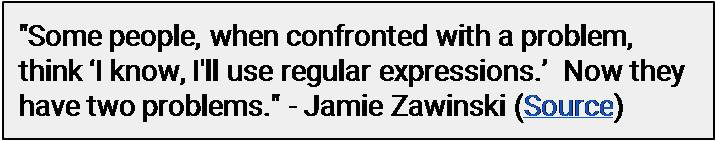
\includegraphics[scale=.7]{Bild14}
        \end{figure}
        \end{column}
         \end{columns}
	    Regular expressions sometimes jokingly referred to as a “write only language”.\\
	    Regular expressions are terrible at certain types of problems. Examples:
	    \begin{itemize}
	        \item For parsing a hierarchical structure, such as JSON, use a parser, not a regex!
	        \item Complex features (e.g. valid email address).
	        \item Counting (same number of instances of a and b). (impossible)
	        \item Complex properties (palindromes, balanced parentheses). (impossible)
	    \end{itemize}
	\end{frame}
	
	
	\begin{frame}{Email Address Regular Expression (a probably bad idea)}
	    The regular expression for email addresses (for the Perl programming language):\\
	    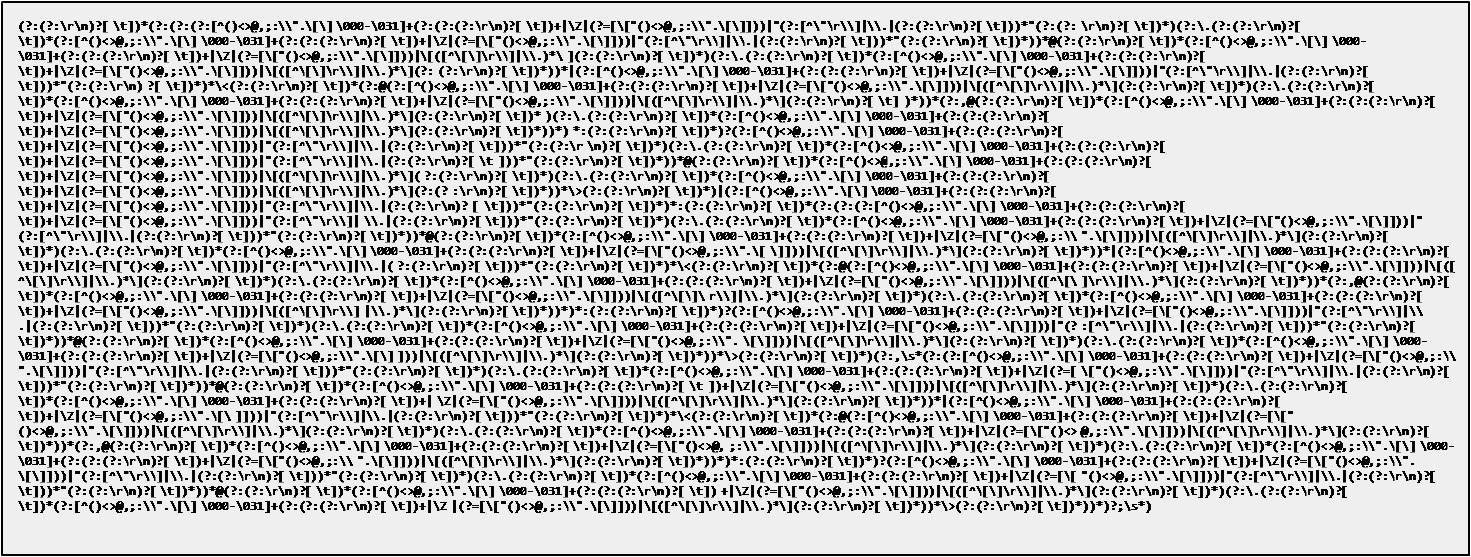
\includegraphics[scale=.58]{Bild15}\\
	    From: \url{http://www.ex-parrot.com/~pdw/Mail-RFC822-Address.html}

	\end{frame}
	
	
	\begin{frame}{Even More Regular Expression Syntax}
	    
	    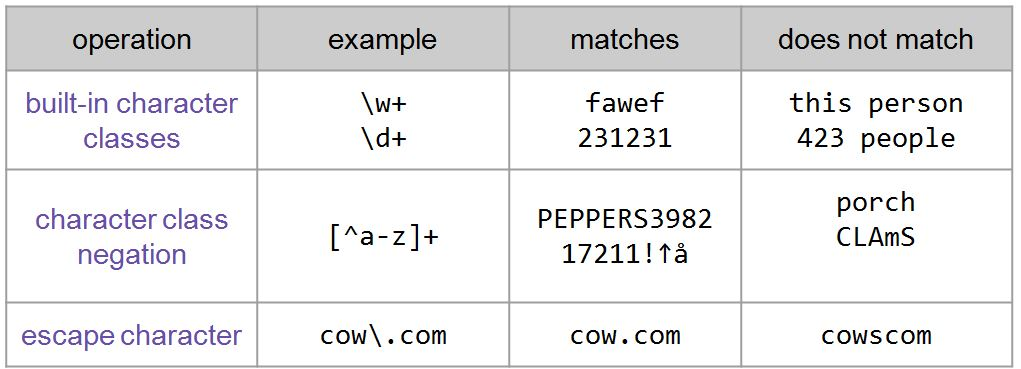
\includegraphics[scale=.45]{Bild16}\\
	    Suppose you want to match one of our special characters like . or [ or ] 
	    \begin{itemize}
	        \item In these cases, you must “escape” the character using the backslash.
	        \item You can think of the backslash as meaning “take this next character literally”.
	    \end{itemize}

	\end{frame}
	
	
	
	\begin{frame}{Regular Expressions Puzzle: \url{tinyurl.com/reg913a}}
	    
	    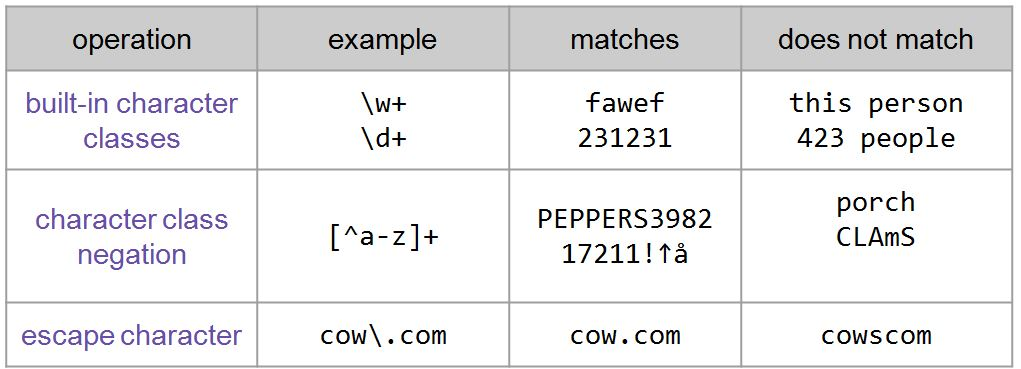
\includegraphics[scale=.45]{Bild16}\\
	    Create a regular expression that matches the red portion below.
	    \begin{figure}
	        \centering
	        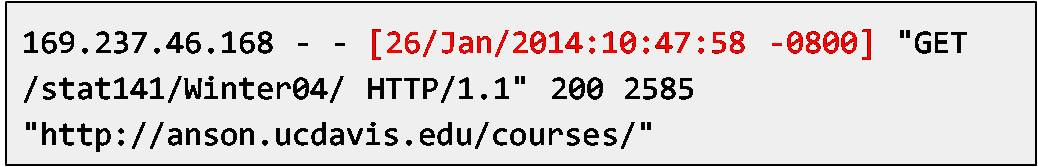
\includegraphics[scale=.5]{Bild17}
	    \end{figure}

	\end{frame}
	
	
	
	\begin{frame}{Regular Expressions Puzzle Solution: \url{tinyurl.com/reg913a}}
	    
	    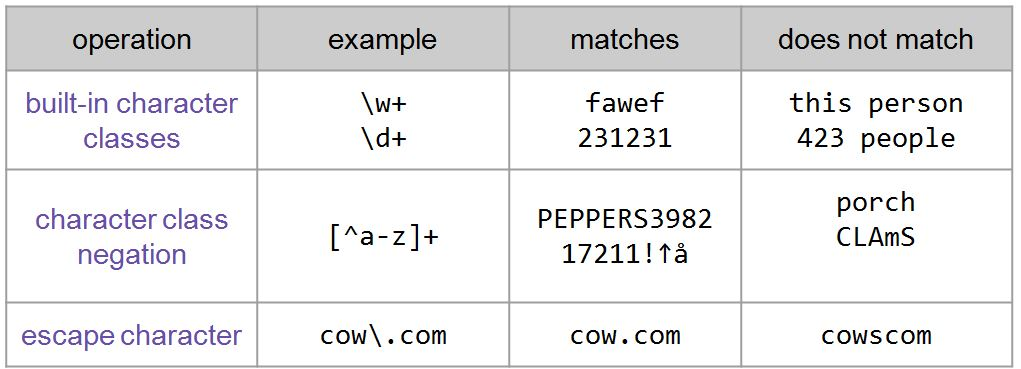
\includegraphics[scale=.45]{Bild16}\\
	    Create a regular expression that matches the red portion below: \textbackslash[.* \textbackslash]
	    \begin{figure}
	        \centering
	        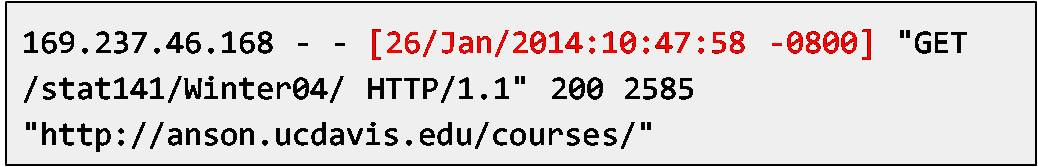
\includegraphics[scale=.5]{Bild17}
	    \end{figure}

	\end{frame}
	
	
	
	\begin{frame}{Quiz \url{tinyurl.com/reg913a}}
	 
	    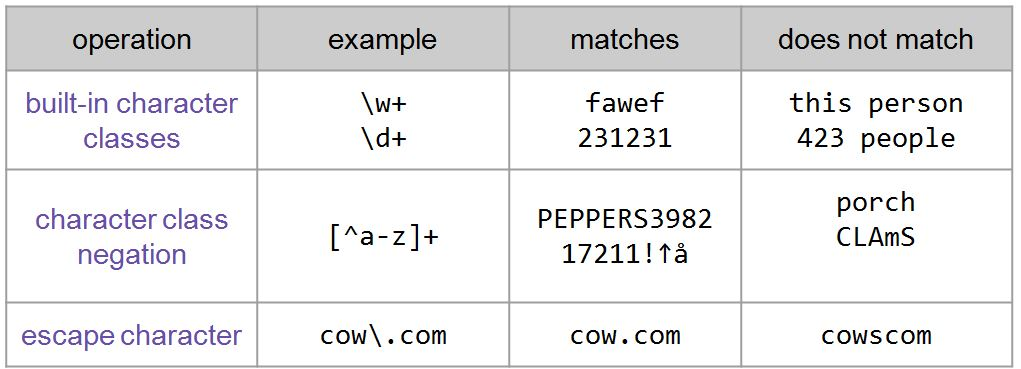
\includegraphics[scale=.43]{Bild16}\\
	    Create a regular expression that matches anything inside of angle brackets <>, but none of the string outside of angle brackets.
        \begin{itemize}
            \item Example: <div><td valign="top">Moo</td></div>
            \item Moo should not match because it is not between < and >.
            \item Note: This is equivalent to the problem of matching HTML tags.
        \end{itemize}

	\end{frame}
	
	
	
	\begin{frame}{Even More Regular Expression Features}
	    \begin{figure}
	        \centering
	        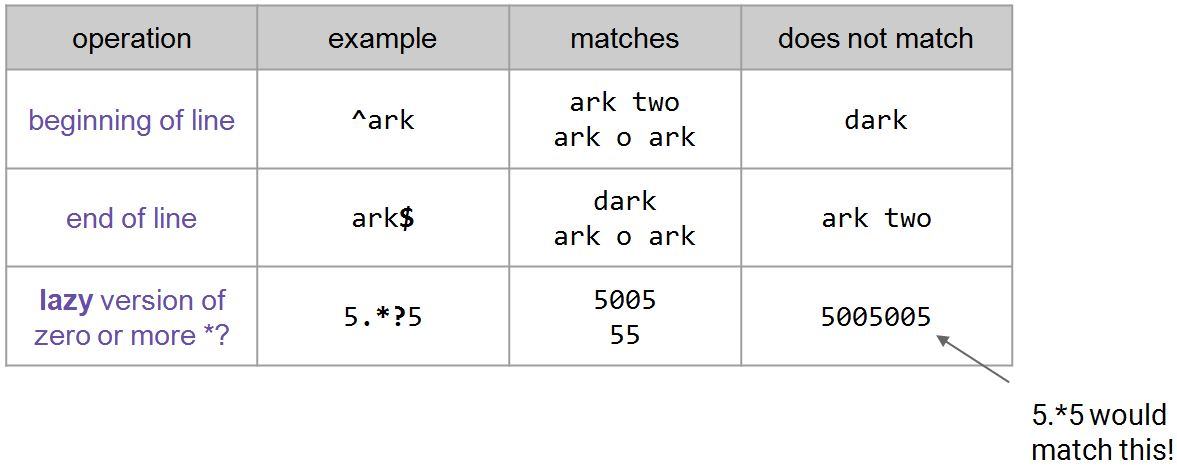
\includegraphics[scale=.35]{Bild18}
	    \end{figure}
	    A few additional common regex features are listed above.
        \begin{itemize}
            \item Won’t discuss these in class, but might come up in discussion or hw.
            \item There are even more out there!
        \end{itemize}
        The official guide is good! \url{https://docs.python.org/3/howto/regex.html}
	\end{frame}
\end{document}